\documentclass[12pt, a4paper]{article} %mostra o tipo do documento
\setlength{\topmargin}{-.5in}
\setlength{\textheight}{9in}
\setlength{\textwidth}{6.3in}
\setlength{\oddsidemargin}{-.125in}
\setlength{\evensidemargin}{-.125in}
\usepackage[brazil]{babel} % permite escrever em português
\usepackage[utf8]{inputenc}
\usepackage[T1]{fontenc} % define a fonte das letras
\usepackage{amsmath, amssymb, amsthm, amsfonts} % permite fazer textos matemáticos
\usepackage{float} % permite mover tabelas e figuras para qualquer ponto da página
\usepackage{graphicx} % permite colocar imagens no documento
\usepackage{color} % permite colorir o texto
\usepackage{listings}

\definecolor{dkgreen}{rgb}{0,0.6,0}
\definecolor{gray}{rgb}{0.5,0.5,0.5}
\definecolor{mauve}{rgb}{0.58,0,0.82}

\newcommand\keywordstyle[1]{{\small\bfseries{#1}}}

\lstset{
    literate=
        {então}{{\keywordstyle{ent\~{a}o}}}5
        {faça}{{\keywordstyle{fa\c{c}a}}}4
        {senão}{{\keywordstyle{sen\~{a}o}}}5
        {até}{{\keywordstyle{at\'{e} }}}4
        {\&\&}{{\keywordstyle{e }}}2
        {lceil}{{$\lceil$}}1
        {rceil}{{$\rceil$}}1
        {lfloor}{{$\lfloor$}}1
        {rfloor}{{$\rfloor$}}1
        {<=}{{$\leqslant$ }}2
        {<=>}{{$\leftrightarrow$ }}2
        {<-}{{$\leftarrow$ }}2,
    frame=single,
    aboveskip=3mm,
    belowskip=3mm,
    showstringspaces=false,
    columns=flexible,
    basicstyle=\small\ttfamily,
    numbers=left,
    numberstyle=\tiny,
    morekeywords={se, TMERGESORT, para, INTERCALA},
    keywordstyle=\bfseries,
    commentstyle=\color{dkgreen},
    stringstyle=\color{mauve},
    breaklines=true,
    breakatwhitespace=true,
    tabsize=3
}
\renewcommand{\ttdefault}{pcr}


\title{ \textbf{Lista 2 - MAC338}}
\date{}
\author{ \textbf{João Gabriel Basi - $\text{N}^\circ$ USP: 9793801}}

\begin{document}
\maketitle
\begin{enumerate}
\item[\textbf{1.}]
\begin{enumerate}
\item[\textbf{a)}]
Supondo que $n$ é potência de 2 e adotando $n^2$ como representante da classe
$\Theta(n^2)$, temos:
\begin{align*}
T(n) &= 2T\left(\frac{n}{2}\right) + n^2\\
     &= 2\left(2T\left(\frac{n}{2^2}\right) + \frac{n^2}{2^2}\right) + n^2 = 2^2T\left(\frac{n}{2^2}\right) + n^2\left(1 + \frac{1}{2}\right)\\
     &= 2^2\left(2T\left(\frac{n}{2^3}\right) + \frac{n^2}{2^4}\right) + n^2\left(1 + \frac{1}{2}\right) = 2^3T\left(\frac{n}{2^3}\right) + n^2\left(1 + \frac{1}{2} + \frac{1}{2^2}\right)\\
     &= ...\\
     &= 2^kT\left(\frac{n}{2^k}\right) + n^2\sum_{i=0}^{k-1}\frac{1}{2^i} \stackrel{PG}{=} 2^kT\left(\frac{n}{2^k}\right) + 2n^2\left(1-\frac{1}{2^k}\right)
\end{align*}
Supondo $k = \lg n$ e $T(1) = 1$, obtemos:
\begin{align*}
T(n) &= nT(1) + 2n^2\left(1-\frac{1}{n}\right)\\
     &= n + 2n^2 - 2n\\
     &= 2n^2 - n\\
     &= \Theta(n^2)
\end{align*}
Verifcando o resultado:\\
Reescrevendo-o em termos de $k = \lg n$ temos
\begin{align*}
T(2^k) &= 2\cdot (2^k)^2 - 2^k \\
       &= 2^{2k+1} - 2^k
\end{align*}
Para $k = 0$: $T(2^0) = 2^{2\cdot 0 + 1} - 2^0 = 2 - 1 = 1$\\
Para $k \geqslant 1$, supomos que a fórmula vale para $k - 1$. Então, utilizando
a recorrência, temos:
\begin{align*}
T(2^k) &= 2T(2^{k-1}) + 2^{2k} \\
       &= 2(2^{2k-1} - 2^{k-1}) + 2^{2k}\\
       &= 2^{2k} - 2^k + 2^{2k}\\
       &= 2^{2k+1} - 2^k\\
\end{align*}
Portanto concluímos que $T(n) = \Theta(n^2)$.

\item[\textbf{d)}]
Supondo que $n$ é potência de 3 e adotando $n^2$ como representante da classe
$\Theta(n^2)$, temos:
\begin{align*}
T(n) &= 7T\left(\frac{n}{3}\right) + n^2\\
     &= 7T\left(7T\left(\frac{n}{3^2}\right) + \frac{n^2}{3^2}\right) + n^2 = 7^2T\left(\frac{n}{3^2}\right) + n^2\left(1 + \frac{7}{9}\right)\\
     &= 7^2T\left(7T\left(\frac{n}{3^3}\right) + \frac{n^2}{3^4}\right) + n^2\left(1 + \frac{7}{9}\right) = 7^3T\left(\frac{n}{3^3}\right) + n^2\left(1 + \frac{7}{9} + \left(\frac{7}{9}\right)^2\right)\\
     &= ...\\
     &= 7^kT\left(\frac{n}{3^k}\right) + n^2\sum_{i=0}^{k-1}\left(\frac{7}{9}\right)^k \stackrel{PG}{=} 7^kT\left(\frac{n}{3^k}\right) + \frac{9n^2\left(1-\left(\frac{7}{9}\right)^k\right)}{2}
\end{align*}
Supondo $k = \log_3 n$ e $T(1) = 1$ e sabendo que $a^{\log_b c} = c^{\log_b a}$, obtemos:
\begin{align*}
T(n) &= 7^{\log_3 n}T(1) + \frac{9n^2\left(1-\left(\frac{7}{9}\right)^{\log_3 n}\right)}{2}\\
     &= n^{\log_3 7} + \frac{9n^2(1-n^{\log_3 7 - 2})}{2}\\
     &= \frac{2n^{\log_3 7} + 9n^2 - 9n^{\log_3 7}}{2}\\
     &= \frac{9n^2 - 7n^{\log_3 7}}{2}\\
     &= \Theta(n^2)
\end{align*}
Verifcando o resultado:\\
Reescrevendo-o em termos de $k = \log_3 n$ temos
\begin{align*}
T(3^k) &= \frac{9\cdot 3^{2k} - 7\cdot 3^{k\log_3 7}}{2}\\
       &= \frac{3^{2k+2} - 7^{k+1}}{2}
\end{align*}
Para $k = 0$: $T(3^0) = \frac{3^{2\cdot 0 + 2} - 7^{0+1}}{2} = \frac{9 - 7}{2} = 1$\\
Para $k \geqslant 1$, supomos que a fórmula vale para $k - 1$. Então, utilizando
a recorrência, temos:
\begin{align*}
T(3^k) &= 7T(3^{k-1}) + 3^{2k}\\
       &= 7\left(\frac{3^{2k} - 7^k}{2}\right) + 3^{2k}\\
       &= \frac{7\cdot 3^{2k} - 7^{k+1} + 2\cdot 3^{2k}}{2} \\
       &= \frac{3^{2k + 2} - 7^{k+1}}{2}
\end{align*}
Portanto concluímos que $T(n) = \Theta(n^2)$.
\end{enumerate}

\item[\textbf{2.}]
Pseudo-código do merge:
\begin{lstlisting}
TMERGESORT(A, b, e):
    se e-b > 2, então:
        p <- (e-b)/3
        m1 <- b + lceilprceil
        m2 <- b + lceil2*prceil
        TMERGESORT(A, b, m1)
        TMERGESORT(A, m1, m2)
        TMERGESORT(A, m2, e)
        INTERCALA(A, b, m1, m2)
        INTERCALA(A, b, m2, e)
    senão, se e-b == 2 && A[b] > A[b+1], então:
        A[b] <=> A[b+1]
\end{lstlisting}
Pseudo-código do intercala:
\begin{lstlisting}
INTERCALA(A, b, m, e):
    B[0...e-b]
    para i <- 0 até m-b-1 faça:
        B[i] <- A[b+i]
    para i <- m-b até e-b-1 faça:
        B[i] <- A[e+m-b-i-1]
    i <- 0
    j <- e-b-1
    para k <- b até e-1 faça:
        se B[i] <= B[j], então:
            A[k] <- B[i]
            i <- i + 1
        senão
            A[k] <- B[j]
            j <- j - 1
\end{lstlisting}
Análise linha por linha:\\
\begin{minipage}{0.45\textwidth}
INTERCALA
\begin{align*}
&3-6  &= \quad &\Theta(n)\\
&7-8  &= \quad &\Theta(1)\\
&9-15 &= \quad &\Theta(n)\\
\hline
&T(n) &= \quad &\Theta(n) \hspace{3cm}
\end{align*}
\end{minipage}
\hfill
\begin{minipage}{0.45\textwidth}
TMERGESORT
\begin{align*}
&2-5   &= \quad &\Theta(1)\\
&6     &= \quad &T\left(\Big\lceil \frac{n}{3} \Big\rceil\right)\\
&7     &= \quad &T\left(\Big\lceil \frac{n}{3} \Big\rceil\right)\\
&8     &= \quad &T\left(\Big\lfloor \frac{n}{3} \Big\rfloor\right)\\
&9-10  &= \quad &\Theta(n)\\
&11-12 &= \quad &\Theta(1)\\
\hline
&T(n) &= \quad &\Theta(n) + 2T\left(\Big\lceil \frac{n}{3} \Big\rceil\right) + T\left(\Big\lfloor \frac{n}{3} \Big\rfloor\right)\\
\end{align*}
\end{minipage}
\\
A partir das contas acima, chegamos na recorrência
$$T(n) = \Theta(n) + 2T(\Big\lceil \frac{n}{3} \Big\rceil) + T(\Big\lfloor \frac{n}{3} \Big\rfloor)$$
Resolvendo-a para $n$ potência de $3$ e $k = log_3 n$ temos
\begin{align*}
T(n)   &= n + n\log_3 n = \Theta(n\log_3 n)\\
T(3^k) &= 3^k + k3^k
\end{align*}
Verifcando o resultado:\\
Para $k = 0$: $T(3^0) = 3^0 + 0\cdot 3^0 = 1 + 0 = 1$\\
Para $k \geqslant 1$, supomos que a fórmula vale para $k - 1$. Então, utilizando
a recorrência, temos:
\begin{align*}
T(3^k) &= 3T(3^{k-1}) + 3^k\\
       &= 3(3^{k-1} + (k-1)3^{k-1}) + 3^k\\
       &= 3^k + (k-1)3^k + 3^k\\
       &= 3^k + k3^k
\end{align*}
Portando concluímos que o algoritmo é $\Theta(n\log_3 n)$.

\item[\textbf{4.}]
O algoritmo terá duas funções, a DIVIDE e a INTERCALA. A DIVIDE recebrá
uma lista de listas, dividirá a lista em duas partes com quase o mesmo tamanho,
executará DIVIDE em cada parte e devolverá o resultado da INTERCALA entre as
duas listas devolvidas pelas execuções do DIVIDE. A INTERCALA receberá duas
listas ordenadas e devolverá uma lista ordenada com todos os elementos das
listas recebidas.\\
Representando como $a$, $b$, $c$ e $d$ os tamanhos das listas recebidas, temos a
seguinte árvore de recorrência:
\begin{center}
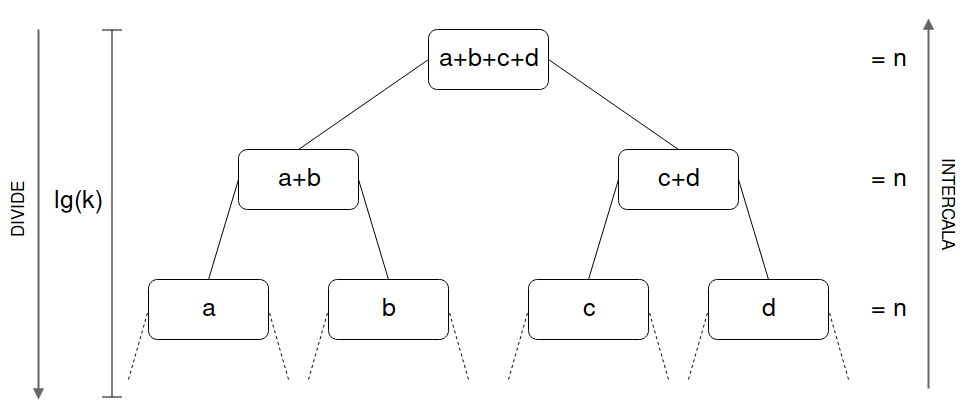
\includegraphics[scale=0.4]{rectree.png}
\end{center}
A cada chamada do DIVIDE, as listas são divididas em dois grupos, o que faz com
que a árvore tenha tamanho médio $\lg k$ e, a cada nível da árvore, o tempo
gasto pelo INTERCALA a cada execução (que está anotado nos quadrinhos da figura)
soma $n$, pois sabemos que $a+b+c+d = n$ e que a INTERCALA é linear. Com isso,
podemos concluir que o algoritmo é $\Theta(n\lg k)$. Em especial se $k = 2$,
a complexidade é $n\lg 2 = n = \Theta(n)$ e se $k = n$ a complexidade é
$n\lg n = \Theta(n\lg n)$.
\end{enumerate}
\end{document}
